\documentclass{article}
\usepackage[utf8x]{inputenc}
\usepackage{ucs}
\usepackage{amsmath} 
\usepackage{amsfonts}
\usepackage{marvosym}
\usepackage{wasysym}
\usepackage{upgreek}
\usepackage[english,russian]{babel}
\usepackage{graphicx}
\usepackage{float}
\usepackage{textcomp}
\usepackage{hyperref}
\usepackage{geometry}
  \geometry{left=2cm}
  \geometry{right=1.5cm}
  \geometry{top=1cm}
  \geometry{bottom=2cm}
\usepackage{tikz}
\usepackage{ccaption}
\usepackage{multicol}

\hypersetup{
   colorlinks=true,
   citecolor=blue,
   linkcolor=black,
   urlcolor=blue
}

\usepackage{listings}
%\setlength{\columnsep}{1.5cm}
%\setlength{\columnseprule}{0.2pt}

\usepackage[absolute]{textpos}

\usepackage{colortbl,graphicx,tikz}
\definecolor{X}{rgb}{.5,.5,.5}


\begin{document}
\pagenumbering{gobble}
\lstset{
  language=C,                % choose the language of the code
  basicstyle=\linespread{1.1}\ttfamily,
  columns=fixed,
  fontadjust=true,
  basewidth=0.5em,
  keywordstyle=\color{blue}\bfseries,
  commentstyle=\color{gray},
  stringstyle=\ttfamily\color{orange!50!black},
  showstringspaces=false,
  numbersep=5pt,
  numberstyle=\tiny\color{black},
  numberfirstline=true,
  stepnumber=1,                   % the step between two line-numbers.        
  numbersep=10pt,                  % how far the line-numbers are from the code
  backgroundcolor=\color{white},  % choose the background color. You must add \usepackage{color}
  showstringspaces=false,         % underline spaces within strings
  captionpos=b,                   % sets the caption-position to bottom
  breaklines=true,                % sets automatic line breaking
  breakatwhitespace=true,         % sets if automatic breaks should only happen at whitespace
  xleftmargin=.2in,
  extendedchars=\true,
  keepspaces = true,
}
\lstset{literate=%
   *{0}{{{\color{red!20!violet}0}}}1
    {1}{{{\color{red!20!violet}1}}}1
    {2}{{{\color{red!20!violet}2}}}1
    {3}{{{\color{red!20!violet}3}}}1
    {4}{{{\color{red!20!violet}4}}}1
    {5}{{{\color{red!20!violet}5}}}1
    {6}{{{\color{red!20!violet}6}}}1
    {7}{{{\color{red!20!violet}7}}}1
    {8}{{{\color{red!20!violet}8}}}1
    {9}{{{\color{red!20!violet}9}}}1
}
\newpage

\title{Семинар \#7: Динамическое выделение памяти.\vspace{-5ex}}\date{}\maketitle
\section*{Указатели}
У каждой переменной есть адрес. Адрес - это номер байта, начиная с которого лежит эта переменная в памяти. Чтобы найти адрес переменной, нужно перед ней поставить знак амперсанда \texttt{\&}. \\
Для хранения адресов в языке C введены специальные переменные, которые называются указатели. Тип переменной указателя = тип той переменной, на которую он `указывает` + звёздочка(\texttt{*}) на конце. Например, указатель, который будет хранить адреса переменных типа \texttt{int} должен иметь тип \texttt{int*}. \\
Чтобы по указателю получить саму переменную, нужно перед указателем поставить звёздочку(\texttt{*}).
\begin{lstlisting}
#include <stdio.h>
int main()
{
    int a = 7;
    printf("Value = %d. Address = %p\n",  a,  &a);
    
    int* pa = &a;
    printf("Value = %d. Address = %p\n", *pa, pa);
}
\end{lstlisting}
Выполните задание из файла \texttt{0pointer\_basics.c}.
\section*{Арифметика указателей}
С указателями можно производить следующие операции:
\begin{itemize}
\item Прибавить или отнять число          \quad             \texttt{p + 2}
\item Вычитать 2 указателя                      \quad       \texttt{p - q}
\item Разыменование (получить то, на что указывает указатель) \quad  \texttt{*p}
\item Квадратные скобки (прибавить число + разыменование): \quad \texttt{p[i] == *(p+i)}
\end{itemize}
Пусть есть одномерный статический массив и указатель на 4-й элемент этого массива:
\begin{lstlisting}
int numbers[6] = {4, 8, 15, 16, 23, 42};
int* p = &numbers[3];
\end{lstlisting}
Чему равны следующие выражения:
\begin{multicols}{3}
\begin{enumerate}
\item \begin{verbatim} numbers[5] \end{verbatim}
\item \begin{verbatim} *p \end{verbatim}
\item \begin{verbatim} *(p+1) \end{verbatim}
\item \begin{verbatim} *(p-2) \end{verbatim}
\item \begin{verbatim} p[0] \end{verbatim}
\item \begin{verbatim} p[1] \end{verbatim}
\item \begin{verbatim} p[-2] \end{verbatim}
\item \begin{verbatim} *numbers \end{verbatim}
\item \begin{verbatim} *(numbers+5) \end{verbatim}
\item \begin{verbatim} p - numbers \end{verbatim}
\item \begin{verbatim} (short*)p - (short*)numbers \end{verbatim}
\item \begin{verbatim} (char*)p - (char*)numbers \end{verbatim}
\end{enumerate}
\end{multicols}
Подсказка: имя массива во многих случаях ведёт себя как указатель на первый элемент массива. \\
Выполните задание из файла \texttt{1pointerarith.c}.

\subsection*{Malloc и free:}
Основные функции для динамического выделения памяти:
\begin{itemize}
\item \texttt{void* malloc(\textbf{size\_t} n)} -- выделяет n байт и возвращает указатель \texttt{void*}
на начало этой памяти \\
\item \texttt{void free(\textbf{void*} p)} -- освобождает выделенную память\\
\item \texttt{void* realloc (\textbf{void*} p, \textbf{size\_t} new\_n)} -- перевыделяет выделенную память\\
\end{itemize}
\begin{lstlisting}
#include <stdio.h>
#include <stdlib.h>

int main()
{
	// Выделяем 50 байт памяти, адрес первого байта будет храниться в указателе p
	void* p = malloc(50); 
	
	// Освободим только - что выделенные 50 байт
	// Память можно освободить в люой момент выполнения, экономя память
	free(p);              

	// Выделяем 12 байт памяти, с указателем p1 теперь
	//       можно обращаться как с массивом размера 3
	int* p1 = malloc(12); 
    
	// Выделяем объём памяти достаточный для хранения 15 - ти int - ов
	int* p2 = malloc(15 * sizeof(int)); 

	// Теперь с p1 и p2 можно работать также как и с массивами типа int
	// То есть можно применять операции типа p1[2]
	// И p1 и p2 будут вести себя как массива размера 3 и 15 соответственно
	for (int i = 0; i < 3; ++i)
		scanf("%d", &p1[i]);
	printf("%d", p1[0] + p1[2]);
	
	// Увеличим размер нашего массива с 15 до 25-ти
	p2 = realloc(p2, 25 * sizeof(int)); 
	
	// Не забывайте освобождать ненужную память!
	free(p1);
	free(p2);
}
\end{lstlisting}


\subsubsection*{Задачи:}
\begin{itemize}
\item Выделить 123 байта памяти и записать адрес на эту память в указатель типа \texttt{void*}.
\item Выделить память для хранения 10 элементов типа \texttt{unsigned long long}.
\item Выделить память для хранения 100 элементов типа \texttt{float*}.
\item Выделить память для хранения 10 элементов типа \texttt{double}. Изменить размер этого динамического массива с 10 до 50, используя \texttt{realloc}.
\item Освободить всю память, которую вы выделили.
\end{itemize}

\newpage
\subsection*{Стек}
\begin{multicols}{2}
\begin{lstlisting}
#include <stdio.h>
struct stack
{
    int n;
    int values[100];
};
typedef struct stack Stack;

void stack_push(Stack* s, int x)
{
    s->values[s->n] = x;
    s->n += 1;
}

int main()
{
    Stack a;
    a.n = 0;
    stack_push(&a, 4);
    stack_push(&a, 10);
    stack_pop(&a);
    printf("%d\n", stack_pop(&a));
}

\end{lstlisting}
\quad\\
\\
\\
\\
\\
\\
Стек — абстрактный тип данных, представляющий собой список элементов, организованных по принципу «последним пришёл — первым вышел». \\

Реализация с помощью массива:

\begin{center}
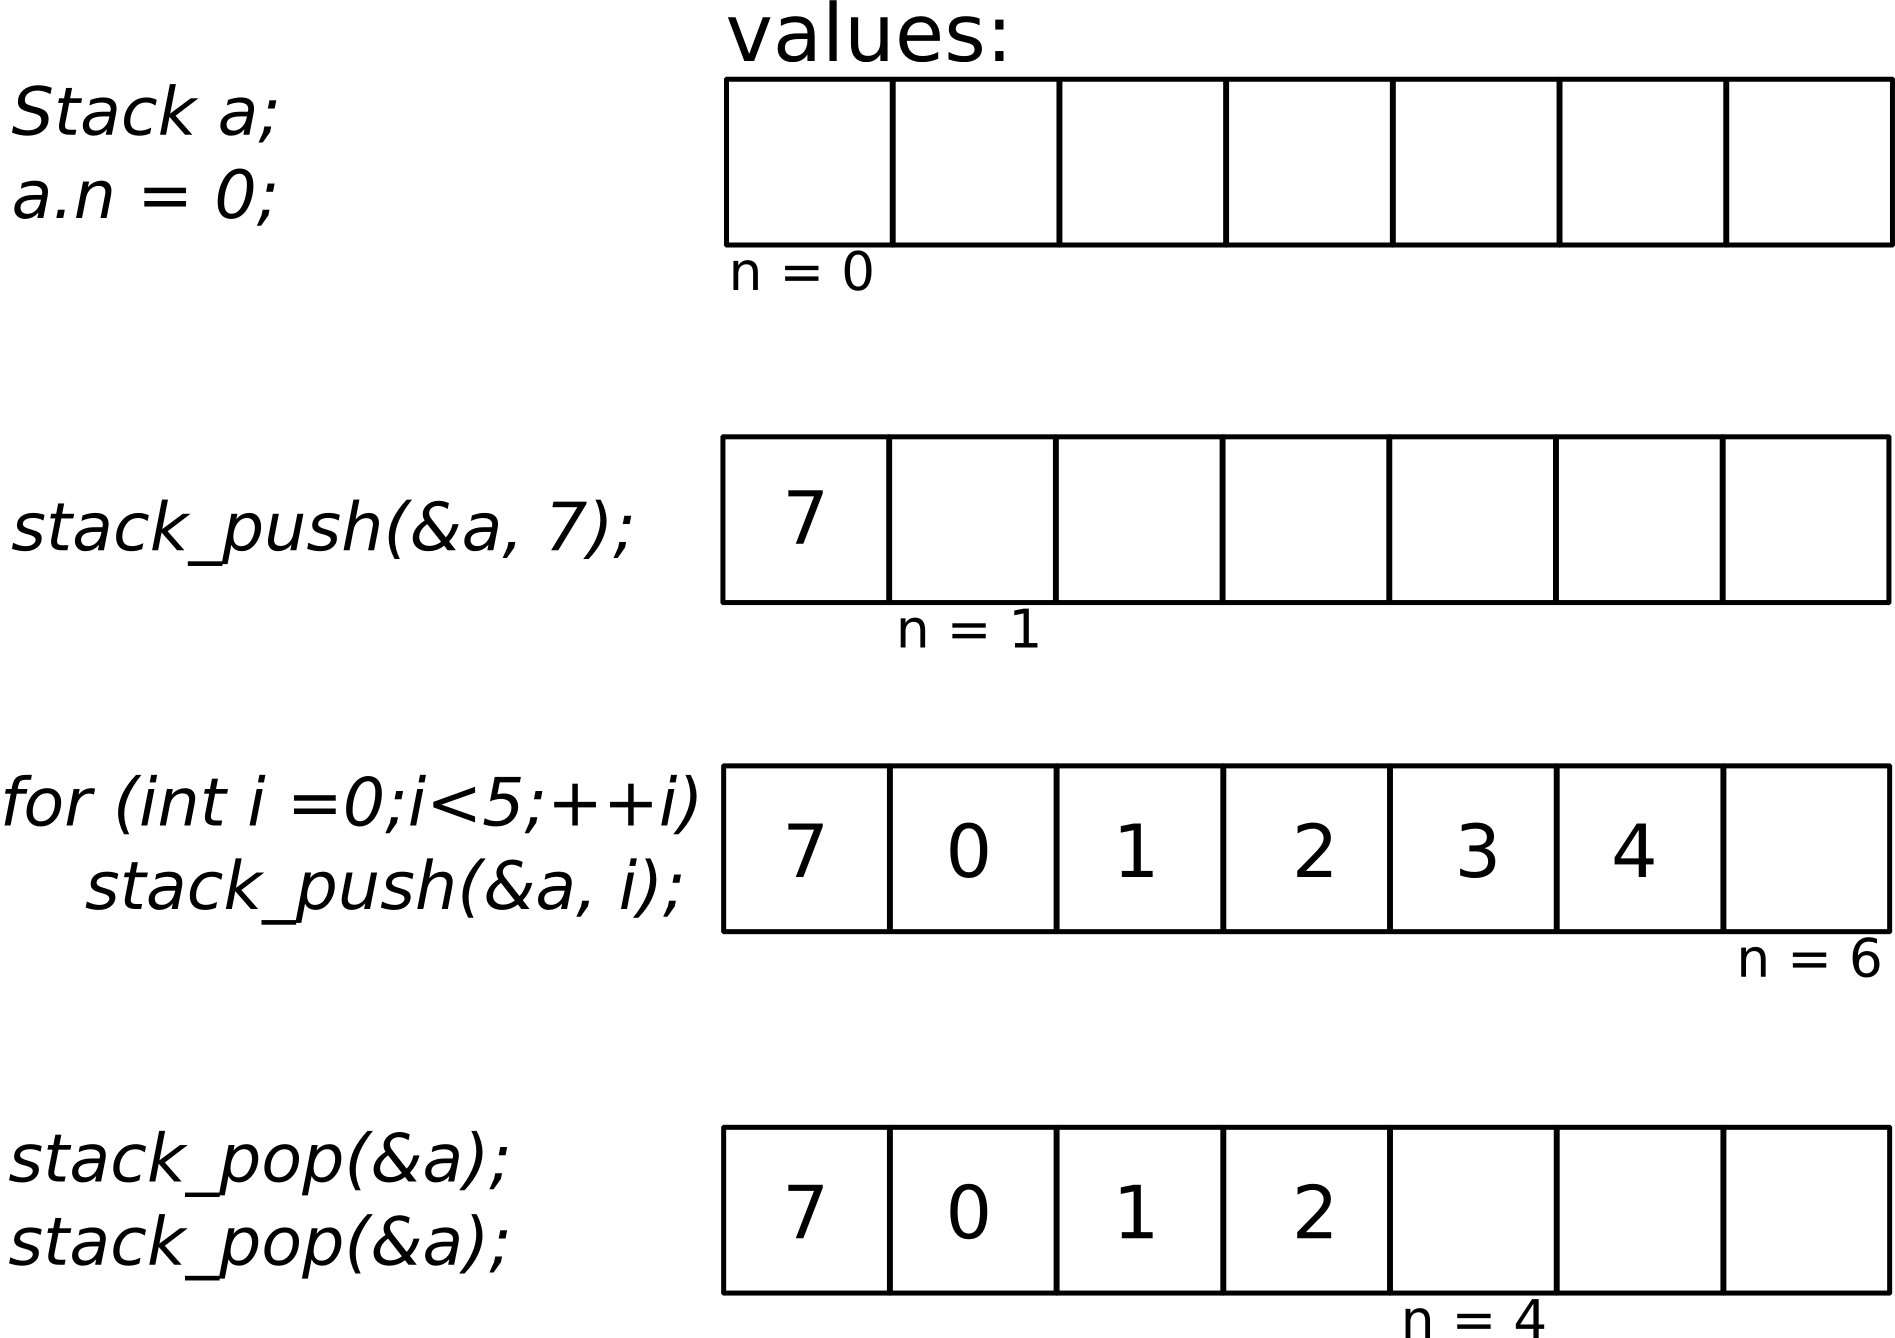
\includegraphics[width=0.95\linewidth]{../images/stack.png}
\end{center}
\end{multicols}

\subsubsection*{Задачи:}
\begin{enumerate}
\item Написать функцию \texttt{int stack\_pop(Stack* s, int x)}. Протестируёте стек: проверьте, что выведет программа, написанная выше.
\item Написать функцию \texttt{int stack\_is\_empty(const Stack* s)}, которая возвращает 1 если стек пуст и 0 иначе.
\item Написать функцию \texttt{int stack\_get(const Stack* s)}, которая возвращает элемент, находящийся в вершине стека, но не изменяет стек.
\item Написать функцию \texttt{void stack\_print(const Stack* s)}, которая распечатывает все элементы стека.
\item Одна из проблем текущей реализации: размер массива 100 задан прямо в определении структуры. Если мы решим изменить максимальный размер стека, то придётся изменять это число по всему коду программы.  Чтобы решить эту проблему введите \texttt{\#define}-константу \texttt{CAPACITY}:
\begin{lstlisting}
#define CAPACITY 100
\end{lstlisting}
\item Что произойдёт, если вызвать \texttt{stack\_push()} при полном стеке? Обработайте эту ситуацию. Программа должна печатать сообщение об ошибке и завершаться с аварийным кодом завершения. Чтобы завершить программу таким образом можно использовать функцию \texttt{exit()} из библиотеки \texttt{stdlib.h}. Пример вызова: \texttt{exit(1)};
\item Аналогично при вызове \texttt{stack\_pop()} и \texttt{stack\_get()} при пустом стеке.
\item Введите функцию \texttt{stack\_init()}, которая будет ответственна за настройку стека сразу после его создания. В данном случае, единственное, что нужно сделать после создания стека это занулить n.
\item Предположим, что вы однажды захотите использовать стек не для целочисленных чисел типа \texttt{int}, а для какого-нибудь другого типа (например \texttt{char}). Введите синоним для типа элементов стека:
\begin{verbatim}
typedef int Data;
\end{verbatim}
Измените тип элемента стека во всех функциях с \texttt{int} на \texttt{Data} (тип поля \texttt{n} менять не нужно). Теперь вы в любой момент сможете изменить тип элементов стека, изменив лишь одну строчку.
\item Сложные скобки. Решить задачу определения правильной скобочной последовательности, используя стек символов. Виды скобок: () \{\} [] <>. Пример неправильной последовательности: (\{<\}>)
\item Стек с динамическим выделением памяти. Описание такого стека выглядит следующим образом:
\begin{verbatim}
struct stack
{
    int capacity;
    int n;
    Data* values;
};
typedef struct stack Stack;
\end{verbatim}
Введено новое поле capacity. В нём будет хранится количество элементов стека, под которые уже выделена память. В отличии от предыдущего варианта стека, это значение будет меняться. \\
values теперь не статический массив, а указатель. Вы должны выделить необходимое место для стека в функции \texttt{stack\_init()}. Начальное значение capacity можно выбрать самостоятельно либо передавать на вход функции \texttt{stack\_init()}. При заполнении стека должно происходить перевыделение памяти с помощью функции \texttt{realloc}.
\end{enumerate}

\end{document}